\chapter{Zusammenarbeit und soziale Funktion}
\textit{Bei PUMA kommt die soziale Komponente natürlich nicht zu kurz. Ob in gemeinsamen Gruppen oder als Freunde, in PUMA lässt es sich gemeinsam arbeiten.}
\section{Freunde}% Screenshot von beiden Seiten (Menü und nutzerseite)
PUMA bietet den Nutzern die Möglichkeit, sich miteinander zu befreunden. Freundschaften\index{Freunde} ermöglichen das Teilen von Publikationen und Lesezeichen. Wählen Sie bei den Sichtbarkeitseinstellung \enquote{andere} und dann \enquote{friends} aus und schon können Ihre Freunde diesen Eintrag sehen. Ebenso können Ihre Freunde Einträge für Sie sichtbar machen. Einen Überblick über diese Einträge erhalten Sie über den Reiter \enquote{meinPUMA} unter \enquote{Einträge von Freunden}.\newline
PUMA bietet zwei unterschiedliche Wege, um Freunde hinzuzufügen.
\newline
\newline
\underline{Weg 1:}
\begin{enumerate} 
    \item Klicken Sie auf den Nutzernamen. Diesen finden Sie bei allen Einträgen, die der Nutzer erstellt hat.
    \item Sie gelangen auf die Seite des Nutzers, auf der alle seine öffentlichen Einträge zu sehen sind. In der rechten Spalte der Seite wird Ihnen der Benutzer angezeigt. Klicken Sie auf \enquote{Freund hinzufügen}.
\end{enumerate}
\begin{figure}[h!]
 \centering
 \fbox{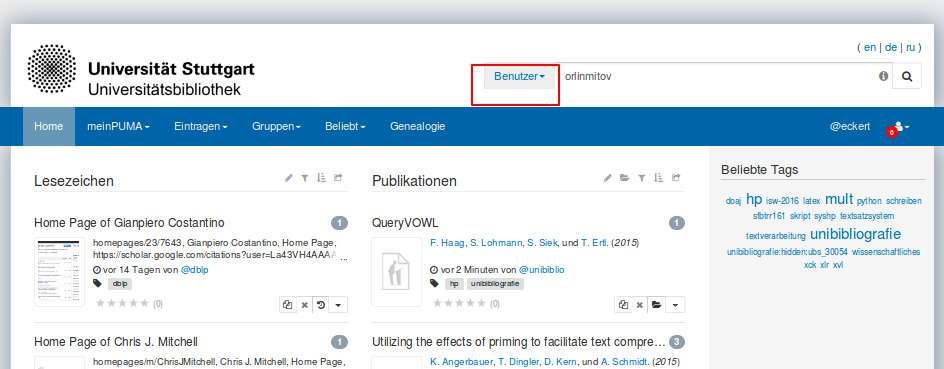
\includegraphics[width=11cm]{Bilder/Kapitel8/Benutzer_suchen}}
 \caption{Benutzer suchen}
 \label{figure057}
\end{figure}
\underline{Weg 2:}
\begin{enumerate}
    \item Wählen Sie in der Suchleiste \enquote{Benutzer} aus und geben den Nutzernamen ein.
    \item Sie gelangen auf die Seite des Nutzers, auf der alle seine öffentlichen Einträge zu sehen sind. In der rechten Spalte der Seite wird Ihnen der Benutzer angezeigt. Klicken Sie auf \enquote{Freund hinzufügen}.
\end{enumerate}
\begin{figure}[h!]
 \centering
 \fbox{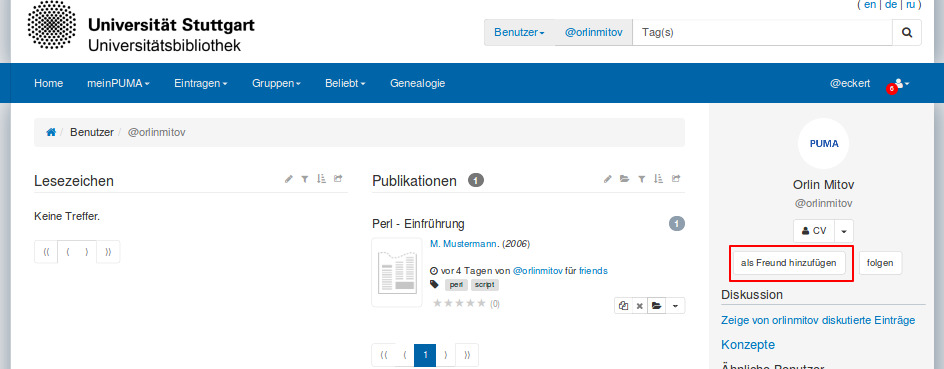
\includegraphics[width=11cm]{Bilder/Kapitel8/Nutzerseite}}
 \caption{Die Nutzerseite}
 \label{figure058}
\end{figure}
\textbf{Freundesübersicht} \newline
Die Freundesübersicht bietet Ihnen einen Überblick über Ihre Freunde in PUMA. Sie gelangen zu der Übersicht über das Dropdown-Menü des Personensymbols. Klicken Sie auf den Reiter \enquote{Freunde}. Sie erhalten nun einen Überblick über Ihre Freunde und können sich auch anschauen, welche Nutzer Sie als Freund angegeben haben. Am Ende der Seite erhalten Sie einen Überblick über alle Publikationen, die Ihre Freunde mit Ihnen oder Sie mit Ihren Freunden teilen.\newline
\begin{figure}[h!]
 \centering
 \fbox{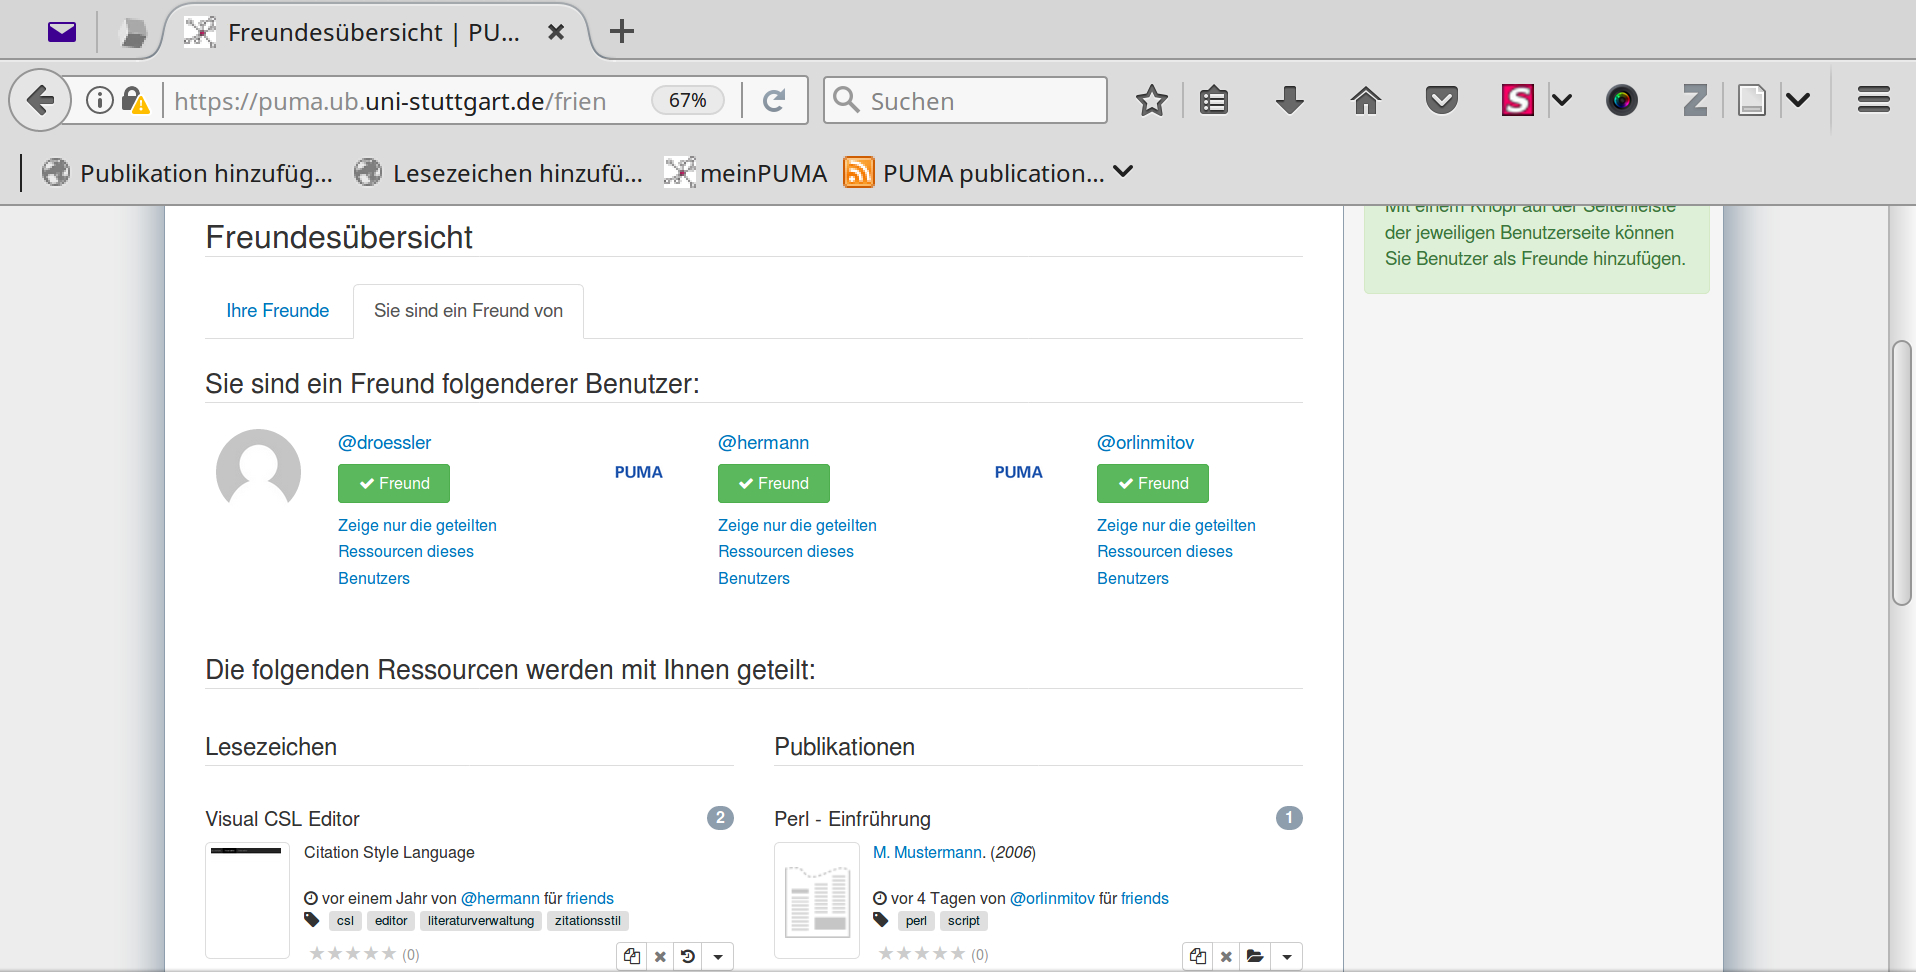
\includegraphics[width=11cm]{Bilder/Kapitel8/Freundesuebersicht}}
 \caption{Freundesübersicht}
 \label{figure059}
\end{figure}
Es besteht jeder Zeit die Möglichkeit Freunde wieder zu entfernen. Gehen Sie hierfür mit der Maus auf den jeweiligen grünen Kasten \enquote{Freund} des Freundes, den Sie entfernen möchten. Der Kasten wird sich von Grün zu Rot verändern und Sie können durch einen Klick auf die linke Maustaste den Freund entfernen. 
\section{Gruppen}
Gruppen\index{Gruppen} vereinfachen die Zusammenarbeit auf Puma. Es ermöglicht eine gemeinsame Literaturrecherche und erleichtert so die Umsetzung von gemeinsamen Projekten. Gleichzeitig kann innerhalb einer Institution/~Arbeitsgruppe der Austausch über neue/~interessante/~fremde/~eigene Artikel mit Hilfe von PUMA erfolgen und somit die Kommunikation vereinfacht werden. 
\subsection{Gruppen \index{Gruppen!beitreten}suchen und beitreten}
\begin{figure}[h!]
 \centering
 \fbox{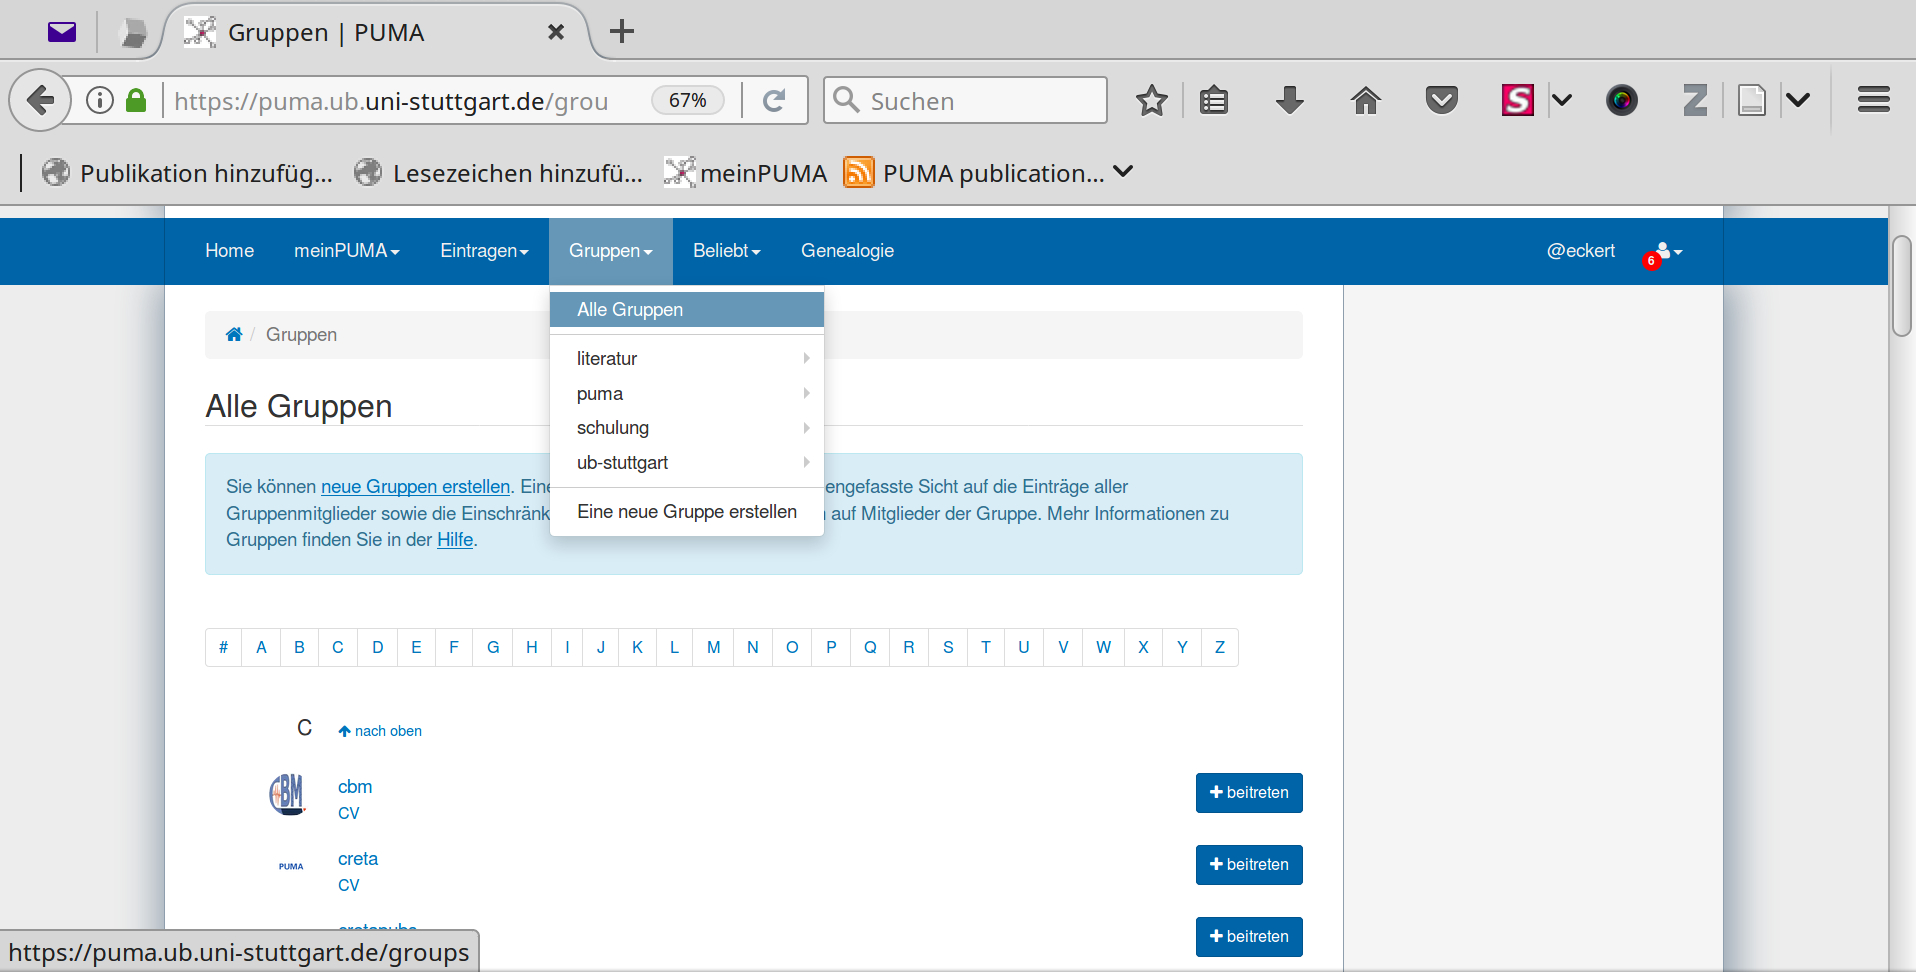
\includegraphics[width=11cm]{Bilder/Kapitel8/Gruppen-Uebersichtsseite}}
 \caption{Allgemeine Liste}
 \label{figure060}
\end{figure}
\begin{enumerate}
    \item Klicken Sie auf \enquote{Gruppen} im Hauptmenü. Ein Dropdwon-Menü öffnet sich.
    \item Klicken Sie im Dropdown-Menü auf \enquote{Alle Gruppen}.
    \item Es öffnet sich eine Übersicht über alle Gruppen bei PUMA in alphabetischer Reihenfolge. Von Links nach Rechts sehen Sie nun den jeweiligen Gruppennamen sowie den Curriculum Vitae von den einzelnen Gruppen. Rechts befindet sich für jede Gruppe ein Button um ihr beizutreten. Klicken Sie auf den entsprechenden Beitreten-Button um der jeweiligen Gruppe beizutreten.
\begin{figure}[h!]
 \centering
 \fbox{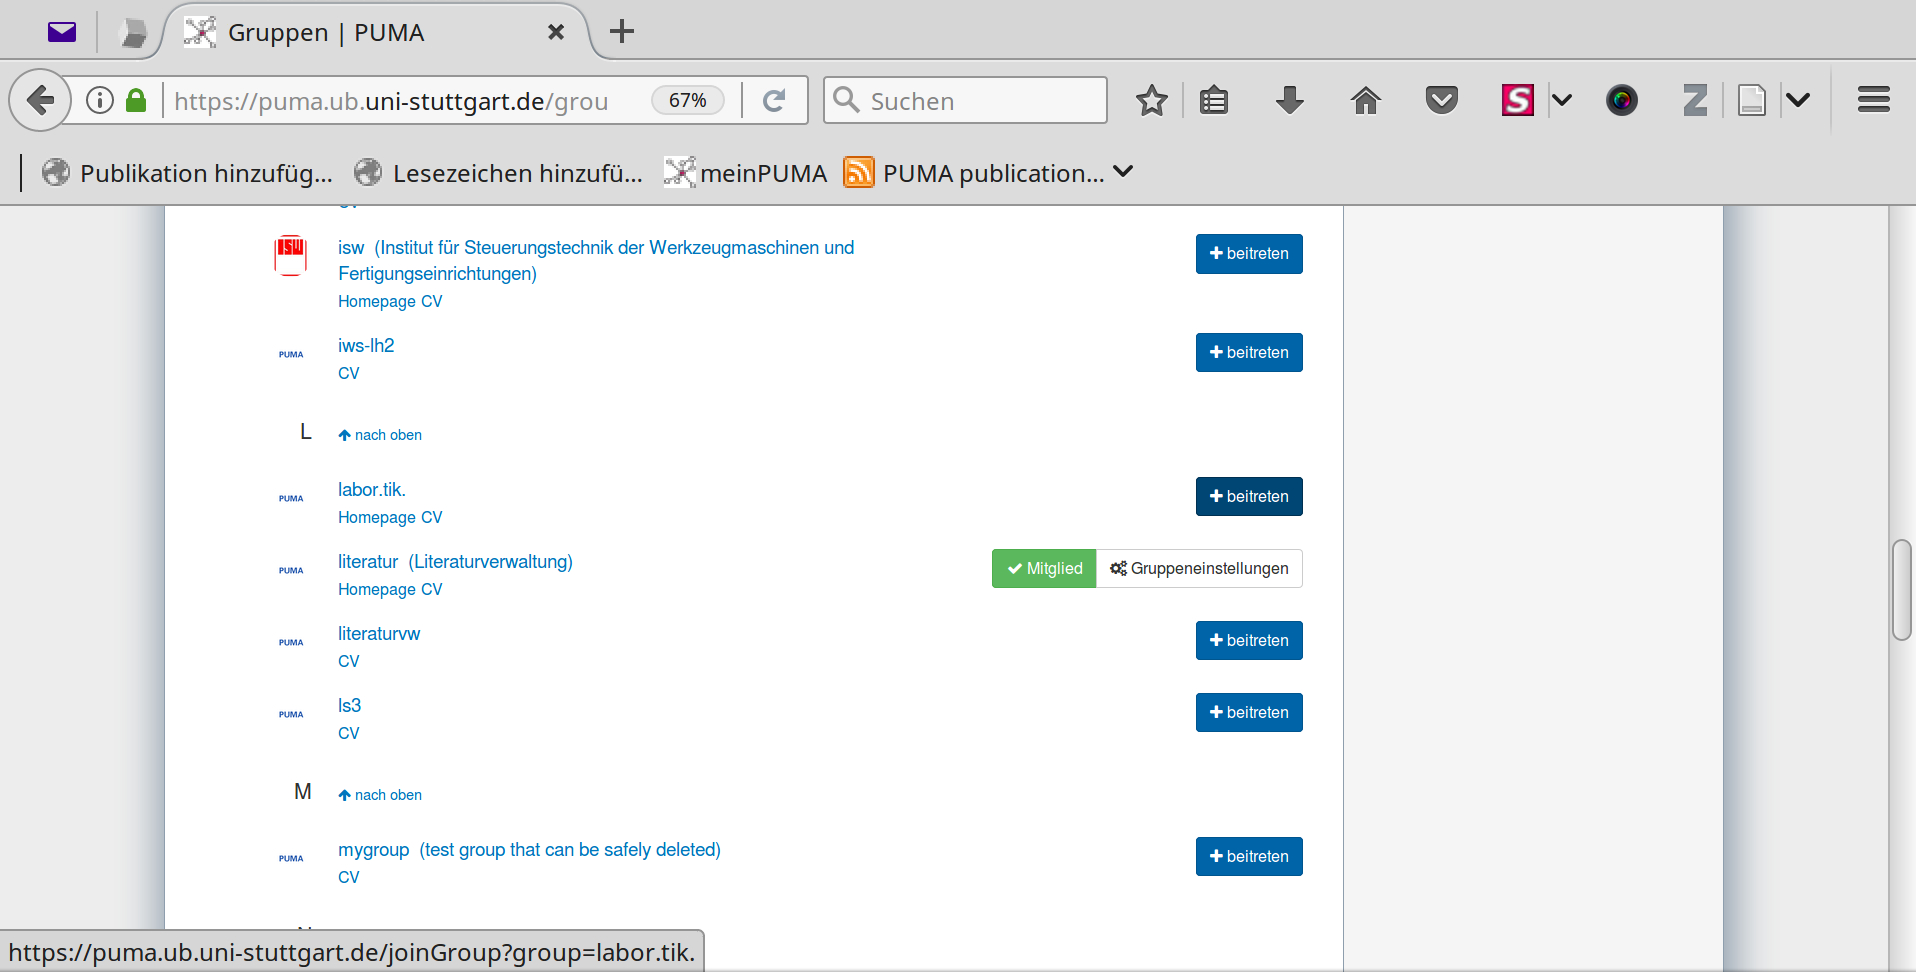
\includegraphics[width=11cm]{Bilder/Kapitel8/Beitreten_einer_Gruppe}}
 \caption{Beitreten einer Gruppe}
 \label{figure061}
\end{figure}
    \item Eine neue Seite erscheint. Geben Sie in das Feld \enquote{Begründung} eine Begründung ein, warum Sie der Gruppe beitreten möchten.
    \item Bitte geben Sie den angezeigten Captcha-Text in das vorgegebene Feld ein, damit wir ausschließen können, dass es sich bei Ihnen um eine Maschine/Roboter handelt.
    \item Klicken Sie anschließend auf \enquote{Anfrage absenden}.
    \item Der Gruppen-Administrator erhält eine E-Mail Benachrichtigung, dass Sie in die Gruppe eintreten wollen. Allein der Administrator entscheidet über die Aufnahme, weswegen ein plausibler Begründungstext sinnvoll ist.
\end{enumerate}
In der E-Mail, die alle Administratoren erhalten, befindet sich ein Link (erster Link in der E-Mail). Durch das Anklicken des Links öffnet sich die Einstellungsseite der Gruppe. Der Administrator kann nun den Nutzer annehmen oder dessen Beitrittsanfrage ablehnen.
\subsection{Gruppen erstellen\index{Gruppen!erstellen}}
\begin{enumerate}
    \item Klicken Sie im Hauptmenü auf \enquote{Gruppen}. Ein Dropdown-Menü öffnet sich.
    \item Klicken Sie im Dropdown-Menü auf \enquote{Eine neue Gruppe erstellen}.
\begin{figure}[h!]
 \centering
 \fbox{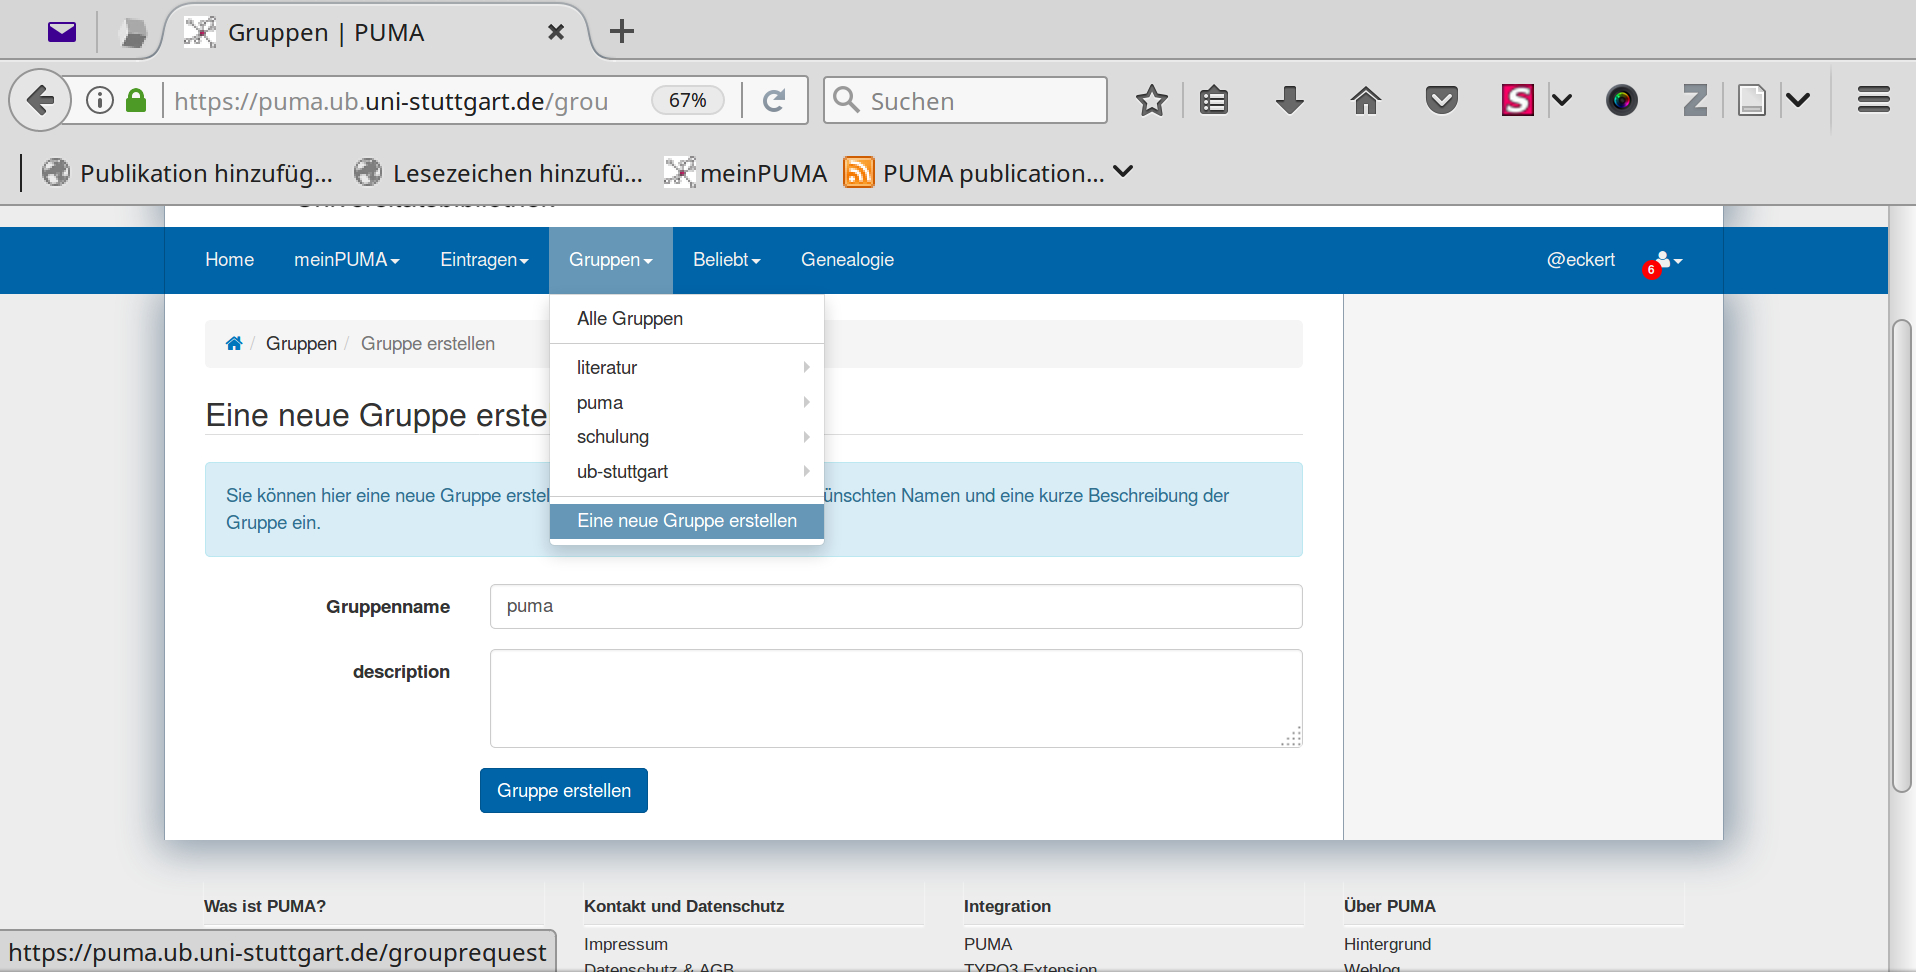
\includegraphics[width=11cm]{Bilder/Kapitel8/Neue_Gruppe_erstellen}}
 \caption{Erstellung einer neuen Gruppe}
 \label{figure062}
\end{figure}
    \item Füllen Sie die freien Felder aus. Erklären Sie bitte auch (unter Begründung) warum bzw. wofür die neue Gruppe genutzt werden soll. Um Spamgruppen zu vermeiden, werden alle Gruppenanträge manuell überprüft. 
    \item Klicken Sie anschließend auf \enquote{Gruppe beantragen}. Der Gruppenantrag wird nun von den Administratoren überprüft. Sobald die Gruppe freigeschaltet wurde, erhalten Sie ein Benachrichtigung per E-Mail.
\end{enumerate}
Ab sofort können Sie die Vorteile der gemeinsamen Literaturrecherche von PUMA nutzen und Publikationen  für spezielle Gruppen sichtbar machen. Dies legen Sie beim Eintragen einer neuen Publikation oder eines neuen Lesezeichen fest, indem Sie bei der Sichtbarkeit\index{Sichtbarkeit} unter dem Punkt \textit{andere} die spezielle Gruppe auswählen. Wenn Sie diese Publikation nun speichern, sehen diese automatisch alle Gruppenmitglieder.
\subsection{Die Gruppenseite}
Um zur Gruppenseite\index{Gruppen} zu gelangen, klicken Sie im Dropdown-Menü vom Reiter  \enquote{Gruppen} auf den entsprechenden Namen der Gruppe. Sie gelangen zur Gruppenseite, auf der Sie einen Überblick über alle Lesezeichen und Publikationen erhalten.%Screenshot
\newline\newline
Funktionen auf der Gruppenseite:
\begin{figure}[h!]
 \centering
 \fbox{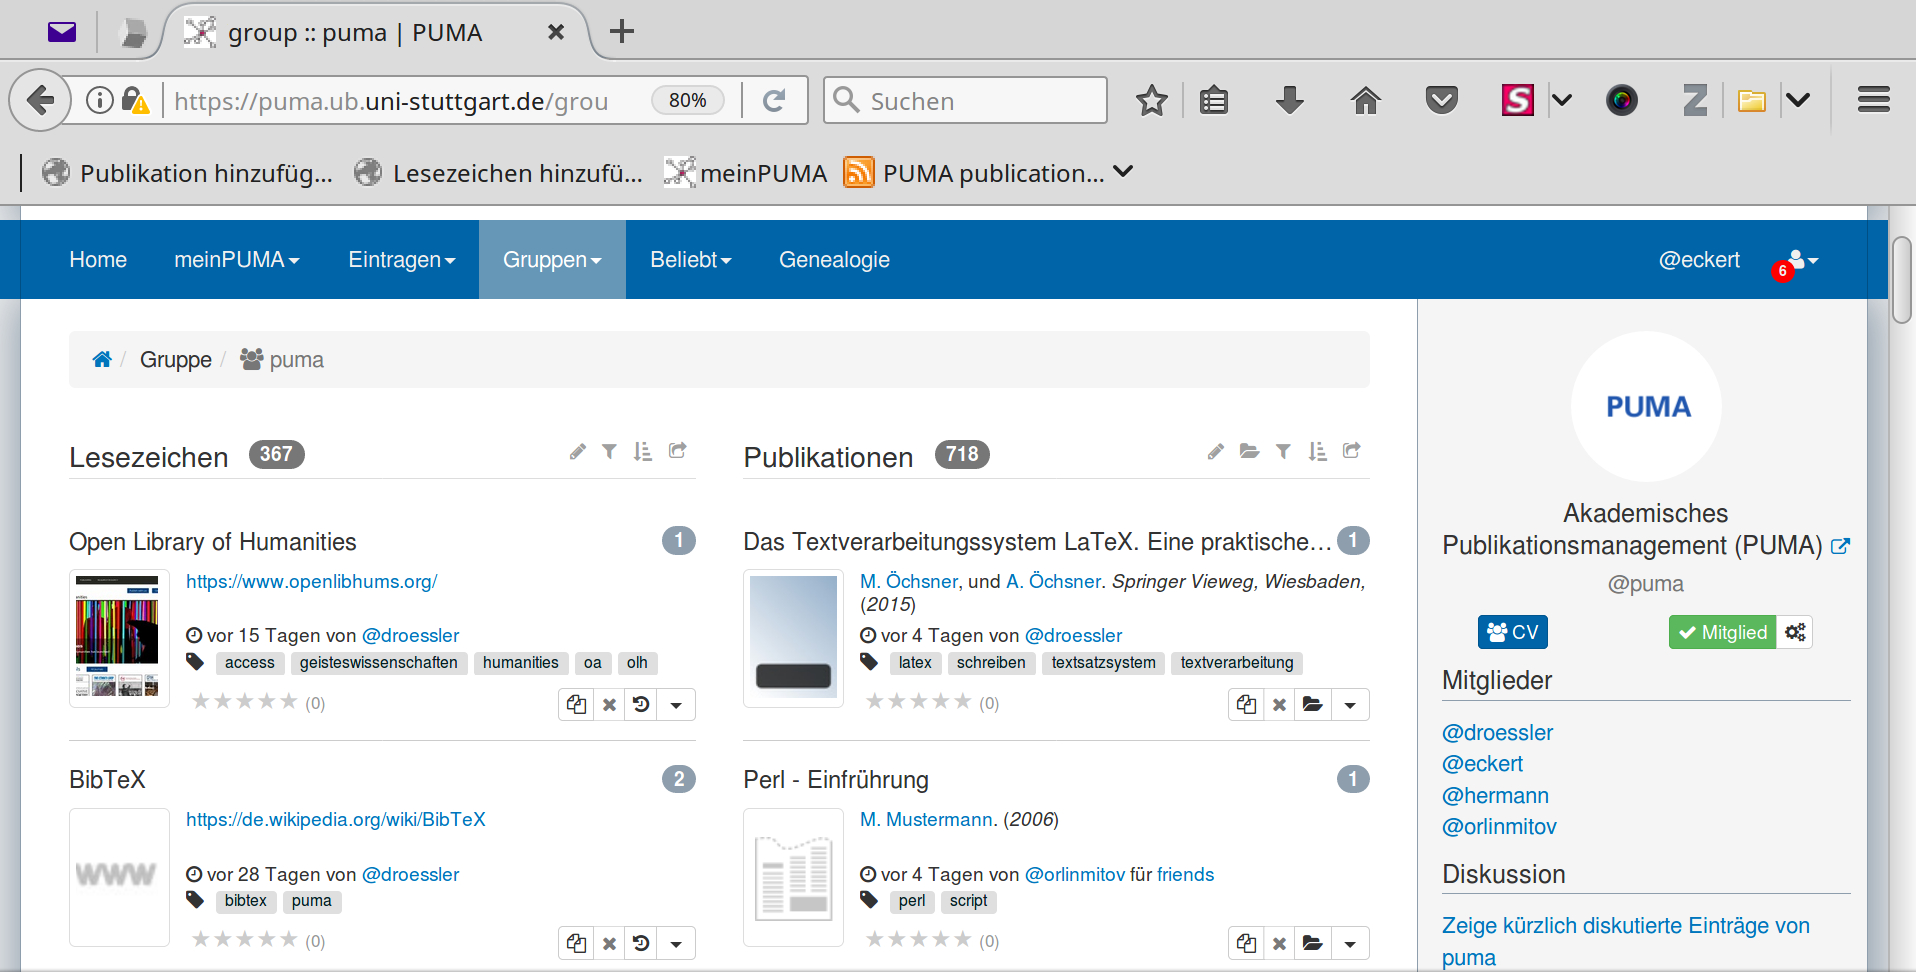
\includegraphics[width=11cm]{Bilder/Kapitel8/Gruppenseite}}
 \caption{Die Gruppenseite}
 \label{figure063}
\end{figure}
\begin{itemize}
\item \textbf{CV/Lebenslauf der Gruppe} finden Sie auf der rechten Seite. Durch Klicken auf den CV-Button erhalten Sie alle wichtigen Informationen zu der Gruppe.
\item Unterhalb des Gruppenbildes befindet sich die \textbf{Liste aller Mitglieder}. 
\item Um sich einen Überblick über die \textbf{diskutierten Einträge} zu verschaffen klicken Sie unter dem Abschnitt Diskussion auf der rechten Seite auf \enquote{Zeige kürzlich diskutierte Einträge von PUMA}. 
\end{itemize}
 
\subsection{Rollen in einer Gruppe}
In einer Gruppe können die unterschiedlichsten Rollen und Aufgaben übernommen werden. In PUMA gibt es drei Rollenarten:
\begin{enumerate}
    \item \underline{Den Administrator}\index{Administrator}: Er hat die größte Befugnis in der Gruppe. Er ist zuständig für die Einstellungen der Gruppenseite und kann das Layout des Gruppenlebenslaufes editieren. Einträge, die in die Gruppe eingetragen werden, können von Ihm/Ihr bearbeitet werden. Ebenfalls kann er neue Mitglieder einladen und vorhandene ausladen sowie die Rollen der anderen Mitglieder verändern (z.B. weiteren Administrator ernennen).
    \item \underline{Den Moderator}\index{Moderator}: Er ist eine Stufe unter dem Administrator. Er hat nur Zugriff auf die Mitgliederliste und kann andere Nutzer in die Gruppe einladen und seine eigene Rolle herabsetzen, indem er zu \textit{Nutzer} wechselt.
    \item \underline{Den Nutzer}\index{Nutzer}: Er ist ein Mitglied der Gruppe und hat keine Befugnisse in der Gruppe Änderungen oder neue Einstellungen vorzunehmen.
\end{enumerate}
\subsection{Einträge für eine Gruppe}
Sobald ein Nutzer Mitglied einer Gruppe ist, werden seine Einträge, die öffentlich sind, automatisch in der Sammlung der Gruppe angezeigt. Die anderen Mitglieder können diese Publikation aber nicht bearbeiten. Erst, wenn Sie die Publikation in Ihre eigene Sammlung übertragen, ist eine Bearbeitung möglich. Eine weitere Möglichkeit bietet das Gruppenoptionsfeld. Dieses kann beim Eintragen der Publikation ausgefüllt werden, indem eine Gruppe ausgewählt wird, für die die Publikation interessant ist. Nachteil bei diesem Vorgehen ist ebenfalls, dass die Einträge nicht von den Mitgliedern bearbeitet werden können. Erst eine Aufnahme in die eigene Sammlung mach eine Bearbeitung des Eintrages möglich.\newline  
Damit andere Mitglieder (Administratoren) einen Eintrag bearbeiten können, muss beim Eintragen der Publikation der Systemtag \textit{for:gruppenname} eingegeben werden. Der Eintrag erscheint wie alle anderen Einträge in der Sammlung der Gruppe. Als Nutzer, der den Eintrag gemacht hat, wird der Gruppenname (@gruppenname) angegeben . In der Reihe der Tags erscheint der Systemtag \textit{from:Benutzername}, welcher den genauen Verfasser des Eintrags angibt. In der Detailansicht der Publikation erhalten nun die Administratoren der Gruppe die Möglichkeit, über den schwarzen Stift oben rechts, die Publikation zu bearbeiten. Hierfür muss die Publikation nicht erneut in die Sammlung des Administrators eingetragen werden.
\section{Community Post}
Ein Community Post\index{Community Post} ist ein Gemeinschaftseintrag zu dem mehrere Personen Zugriff haben. \newline \newline
\textbf{Erstellen eines Community Posts:}
\begin{enumerate}
	\item Klicken Sie auf den Titel der Publikation und Sie gelangen zur Detailansicht der Publikation. 
	\item Gehen Sie mit der Maus auf den kleinen schwarzen Pfeil oben rechts neben dem Publikationstitel. 
	\item Wählen Sie im Dropdown-Menü \enquote{CommunityPost} aus. \end{enumerate}
\begin{figure}[h!]
 \centering
 \fbox{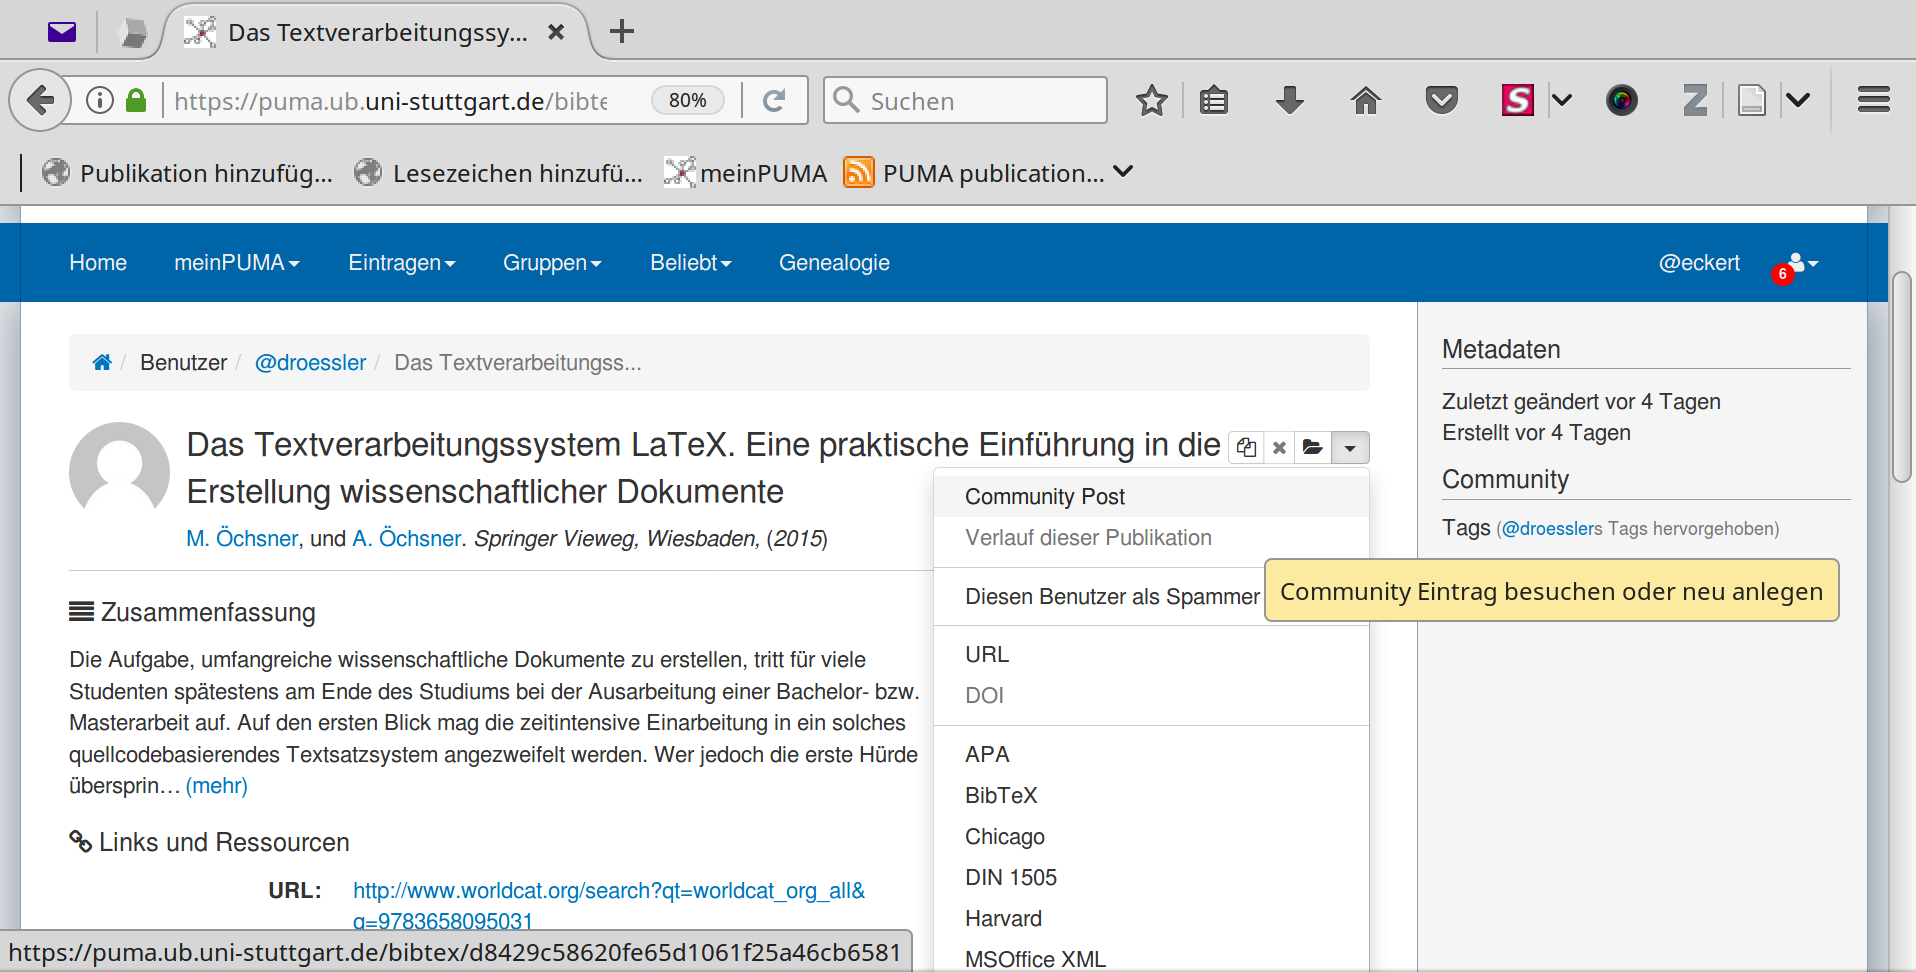
\includegraphics[width=11cm]{Bilder/Kapitel8/Community_post_anlegen}}
 \caption{Community Post anlegen}
 \label{figure064}
\end{figure}
Der Community Post öffnet sich. Sie können nun Änderungen an der Publikation vornehmen, indem Sie oben links auf der Seite auf den Stift klicken, oder weiter unten auf der Community-Seite die Publikation bewerten. Die Änderungen werden in einer Übersicht, der Versionsgeschichte\index{Versionierung}, dargestellt. Zu dieser gelangen Sie oben links, durch Klicke auf das Verzeichnissymbol.\newline
Durch die Erstellung eines Community Post können die Nutzer jederzeit auf die Versionsgeschichte des Eintrages zugreifen und sehen, was und wann von wem geändert wurde. So erleichtert er die Zusammenarbeit und ermöglicht einen umfassenden Überblick. \newline
Im Bereich \textit{Tags} werden einem alle Publikationen mit diesem Tag angezeigt, wenn man auf das entsprechende Tag klickt. \newline
Unter dem Bereich \textit{Nutzer} werden alle Nutzer angezeigt, die diese Publikation in Ihrer Sammlung eingetragen haben.
\begin{figure}[h!]
 \centering
 \fbox{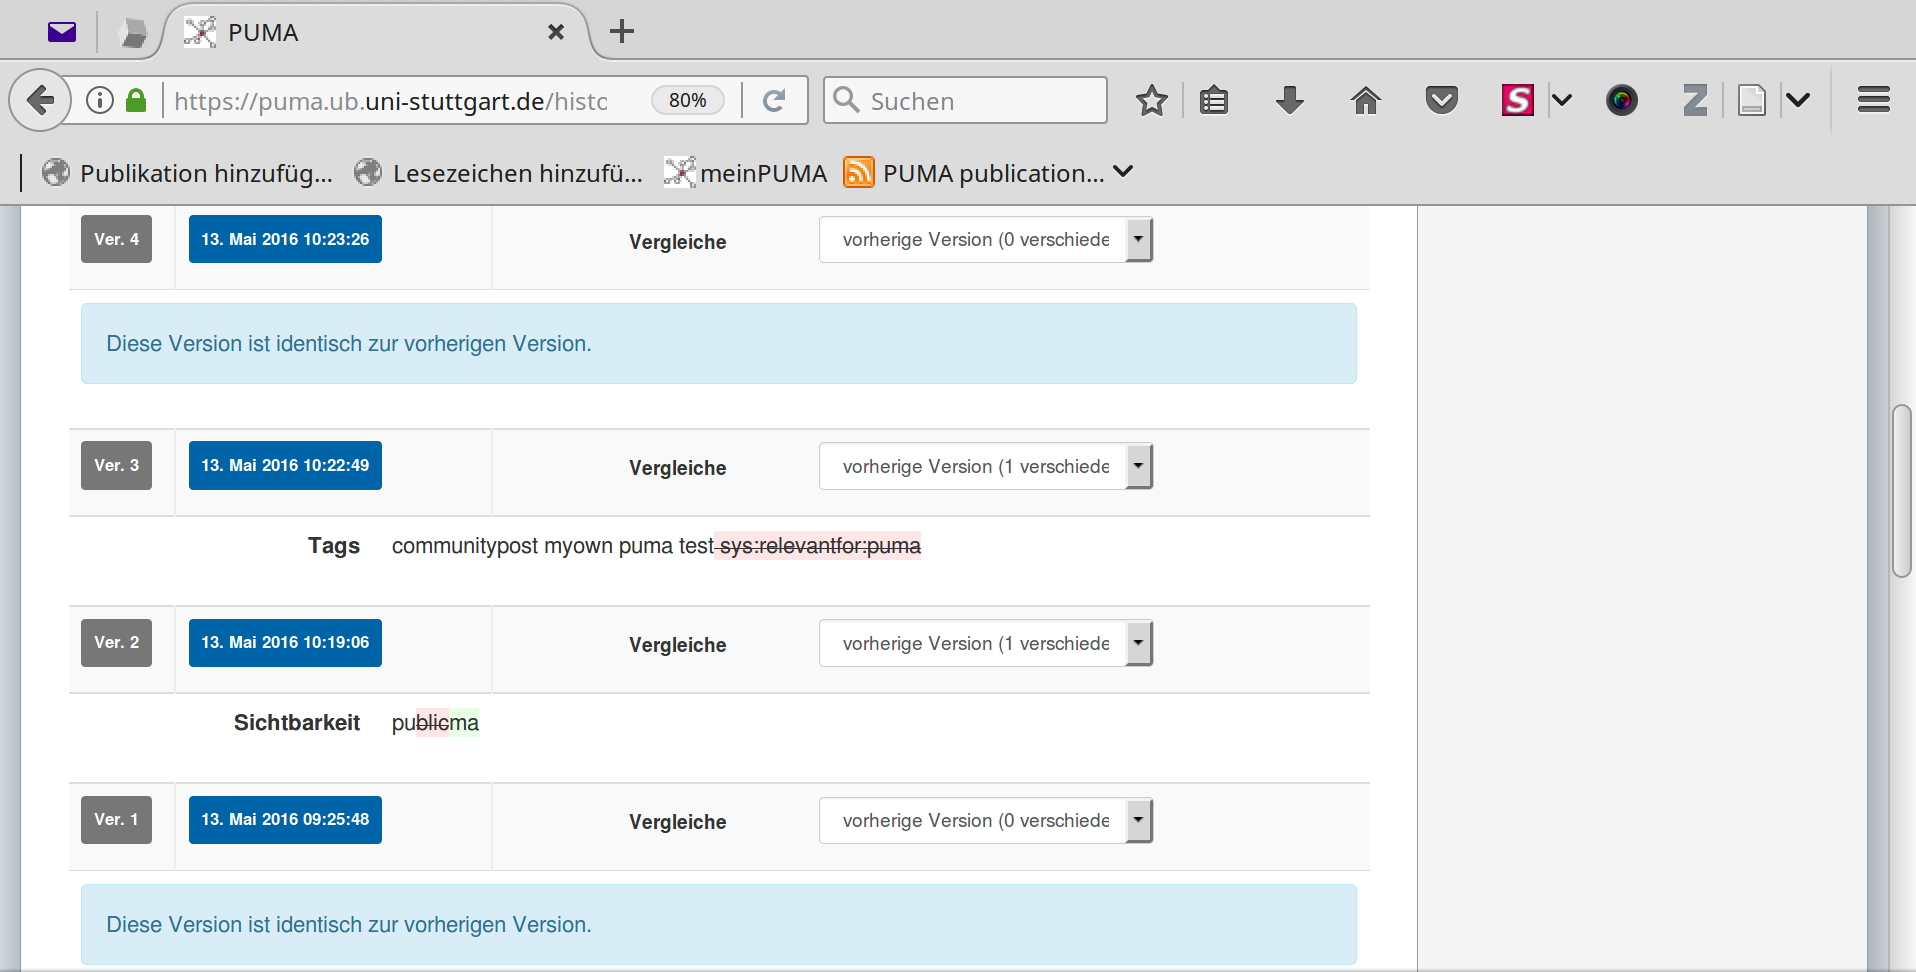
\includegraphics[width=11cm]{Bilder/Kapitel8/Community_post_Versionsgeschichte}}
 \caption{Versionierung}
 \label{figure065}
\end{figure}
\section{Nutzern folgen}
Wie in den sozialen Netzwerken bietet PUMA seinen Nutzern die Möglichkeit anderen Nutzern zu folgen. \newline
Um einem Nutzer zu folgen gehen Sie auf dessen Benutzerseite. Klicken Sie rechts oben, unterhalb des Benutzerprofilbildes, auf das Feld \enquote{folgen}. Ab sofort sind Sie ein Follower des Nutzers. Sie können jedem Nutzer, egal ob befreundet oder nicht, folgen. \newline \newline
Um eine Überblick über die Einträge der verfolgten Person zu erhalten, klicken Sie im Reiter \enquote{meinPUMA} auf den Unterpunkt \enquote{verfolgte Einträge}. Es erscheint eine Übersichtsseite mit alle Einträgen der Nutzer, denen Sie folgen. 




%Überarbeiten:neue version anders

\section{Kommentare, Rezensionen und Bewertungen}
PUMA verfügt über die Möglichkeit Publikationen/~Lesezeichen zu bewerten\index{Bewerten} und Rezensionen\index{Rezensionen} zu verfassen. Man kann mit anderen Nutzern über Publikationen/~Lesezeichen diskutieren und seine eigene Meinung zu einer Publikation/~einem Lesezeichen durch die Vergabe von Sternen verdeutlichen.
\newline
\newline
Publikationen/Lesezeichen bewerten:
\begin{enumerate}
    \item Klicken Sie auf die Stern-Leiste, diese befindet sich unterhalb von jedem Eintrag eines Lesezeichen oder einer Publikation.
\begin{figure}[h!]
 \centering
 \fbox{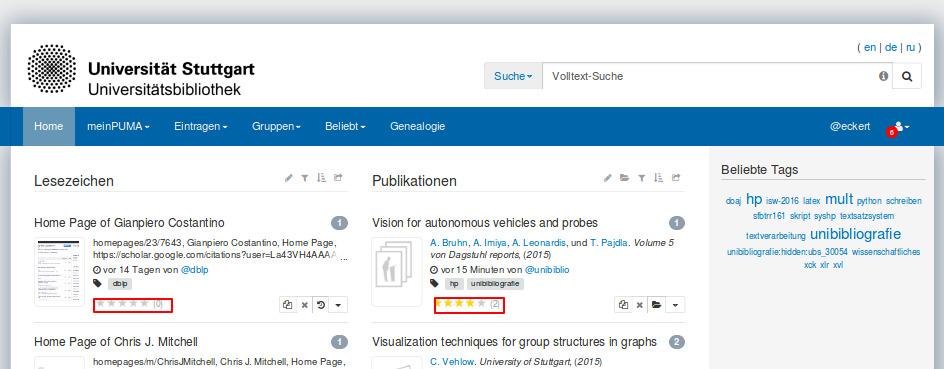
\includegraphics[width=11cm]{Bilder/Kapitel8/Die_Sternenleiste}}
 \caption{Die Sternenleiste}
 \label{figure066}
\end{figure}  
    \item Es öffnet sich die Gemeinschaftsseite des Eintrages. Neben den Bereichen \textit{Tags} und \textit{Zitieren Sie diese Publikation} finden Sie hier auch den Bereich \textit{Kommentare und Rezensionen}. 
\begin{figure}[h!]
 \centering
 \fbox{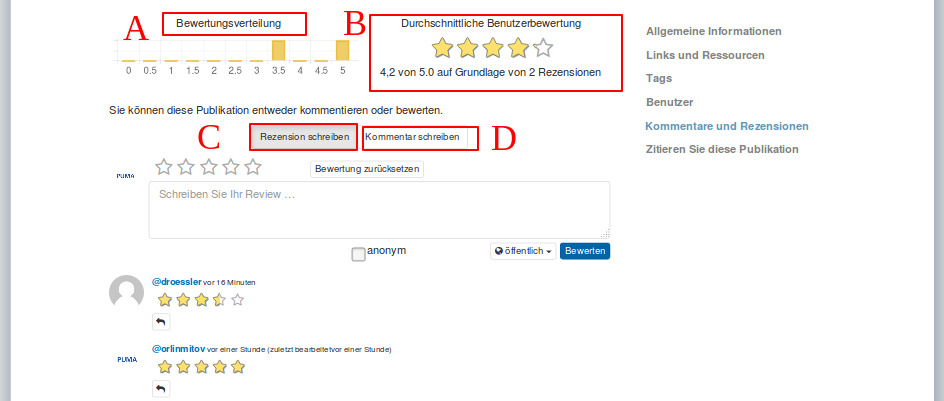
\includegraphics[width=11cm]{Bilder/Kapitel8/Publikation_bewerten}}
 \caption{Publikation bewerten}
 \label{figure067}
\end{figure}
    \begin{itemize} 
        \item \textbf{A (Bewertungsverteilung):} Dies ist ein Balkendiagramm, das alle bisherigen Bewertungen anschaulich darzustellen. %In diesem Fall ... Beispiel an Hand eines Bildes
        \item \textbf{B (Durchschnittliche Bewertung):} In der Stern-Leiste  werden die Bewertungen aus A zusammengefasst.
        \item \textbf{C (Rezension schreiben):} Durch klicken auf den Button öffnet sich ein Textfeld, das Ihnen die Möglichkeit bietet ein Review  zu verfassen. Oberhalb des Textfeldes können Sie den Beitrag auf einer Sternen-Leiste mit 0-5 Sternen bewerten. Je höher die Anzahl der Sterne, umso besser ist die Bewertung. Unterhalb des Textfeldes können Sie die Sichtbarkeit Ihrer Bewertung festlegen und so entscheiden, wer sie alles sehen darf. Es gibt folgende Möglichkeiten:
        \begin{enumerate}
            \item öffentlich: Jeder Nutzer kann Ihre Rezension sehen.
            \item privat: Nur Sie können Ihre Rezension sehen.
            \item Freunde: Sie können bestimmte Freunde festlegen, die Ihre Rezension sehen sollen.
            \item Gruppen: Es werden Ihnen alle Gruppen angezeigt, in denen Sie Mitglied sind. Wählen Sie aus, welche Gruppe die Rezension sehen soll.
            \item anonym: Ihr Kommentar wird ohne Ihren Benutzernamen veröffentlicht. Die Bewertung ist für alle Nutzer sichtbar.
        \end{enumerate}
       	Klicken Sie abschließend auf \enquote{Bewerten} um die Rezension abzuschließen und sie sichtbar zu machen.
        \item \textbf{D (Kommentar schreiben):} In dieses Textfeld haben Sie die Möglichkeit einen Kommentar zu verfassen. Sie können zwischen den gleichen Möglichkeiten der Sichtbarkeit wählen wie unter dem Bereich \enquote{Rezension erstellen}.
\newline Es kann beliebig oft auf Kommentare/~Bewertungen reagiert und geantwortet werden. Neben jedem Kommentar befindet sich ein Button mit einem kleinen schwarzen Pfeil, über ihn können Sie Rezensionen direkt kommentieren. 
    \end{itemize}
\end{enumerate}